% Chapter 3

\chapter{Data} % Main chapter title
\label{data}

\section{Corpus}

The corpus consists of 561 PDF documents published by Novartis. Each trial can have two documents: a technical \emph{Clinical Trial Results} report and a \emph{Patient Summary} written for the public. The documents are treated as non-redistributable; this thesis therefore reports aggregate statistics and quotes at most short fragments of source or model text.

Figure~\ref{fig:funnel} shows how the corpus reduces to usable trials. The 561 PDFs cover 273 protocol IDs. Of these, 256 IDs have both a report and a patient summary, and 17 have only one of the two documents. For 44 of the 256 pairs the PDF parser extracted no sections from one of the documents, because its section detection relies on bold-font headers and differently formatted PDFs come back empty. This leaves \textbf{212 usable trials}, of which 211 yield at least one example.

The abstract of the original thesis reports 286 trials \parencite{barmpas2024pls}. That count cannot be reproduced from this corpus, which holds only 273 distinct protocol IDs; the original count probably used a different pairing or counting rule. All numbers in this thesis refer to the dataset as rebuilt here.

\begin{figure}[htbp]
    \centering
    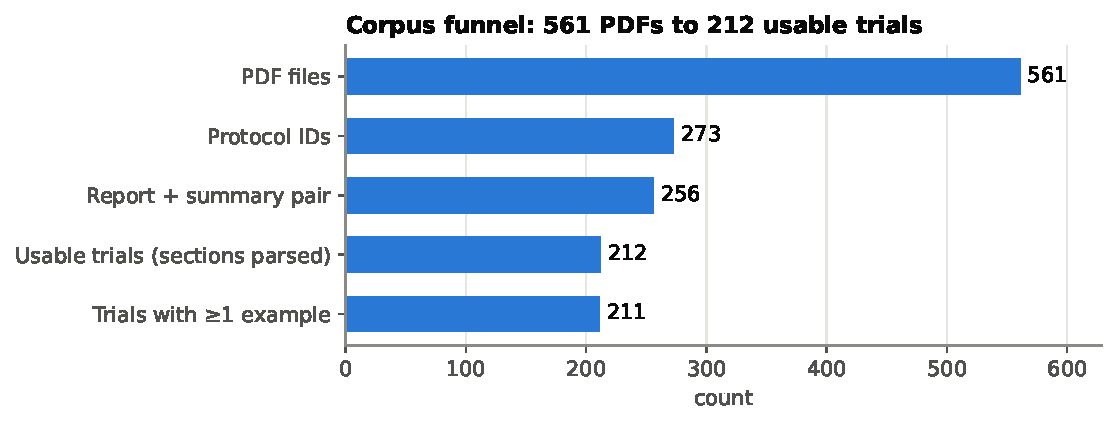
\includegraphics[width=\textwidth]{Figures/results/fig01_corpus_funnel.pdf}
    \caption[Corpus funnel]{From 561 PDFs to 212 usable trials.}
    \label{fig:funnel}
\end{figure}

\section{From Documents to Examples}

Each patient summary answers up to eight canonical patient questions. For every usable trial and question, an example is formed from the question, the report section(s) mapped to that question (the \emph{context}) and the patient-summary section that answers it (the \emph{reference}). The question-to-section mapping is the one defined in the original thesis. An example is dropped when the mapped report section is missing (\emph{no context}) or when the summary does not contain that question (\emph{no answer}).

Table~\ref{tab:coverage} and Figure~\ref{fig:coverage} give the coverage per question. The construction yields \textbf{959 examples}. Coverage is uneven: \emph{What were the results of the trial?} is answered for 201 trials, \emph{How has this trial helped?} for only 87. Most losses are \emph{no answer}, because older patient-summary templates do not ask every question.

\textbf{The adverse-events question contributes no examples.} Its mapped report section, \emph{Trial Analysis}, occurs in none of the 212 parsed reports. The same missing section leaves the treatments question with only \emph{Statistical Methods} as context and the results question with only \emph{Conclusion}. The study therefore evaluates \textbf{7 of the 8 questions}. This is a defect of the inherited mapping, not a property of the task: 179 of the patient summaries do answer the adverse-events question, and the reports contain safety sections that a corrected mapping could use (Section~\ref{sec:future}).

\begin{table}[htbp]
    \centering
    \small
    \caption[Examples per question]{Examples per question and reasons for exclusion (212 usable trials). The mapping of questions to report sections is inherited from the original thesis.}
    \label{tab:coverage}
    \begin{tabularx}{\textwidth}{>{\raggedright\arraybackslash}p{4.6cm}rrr>{\raggedright\arraybackslash}X}
        \toprule
        Question & Usable & No answer & No context & Mapped report sections \\
        \midrule
        \tabinput{Tables/dataset_coverage_body.tex}
        \bottomrule
    \end{tabularx}
\end{table}

\begin{figure}[htbp]
    \centering
    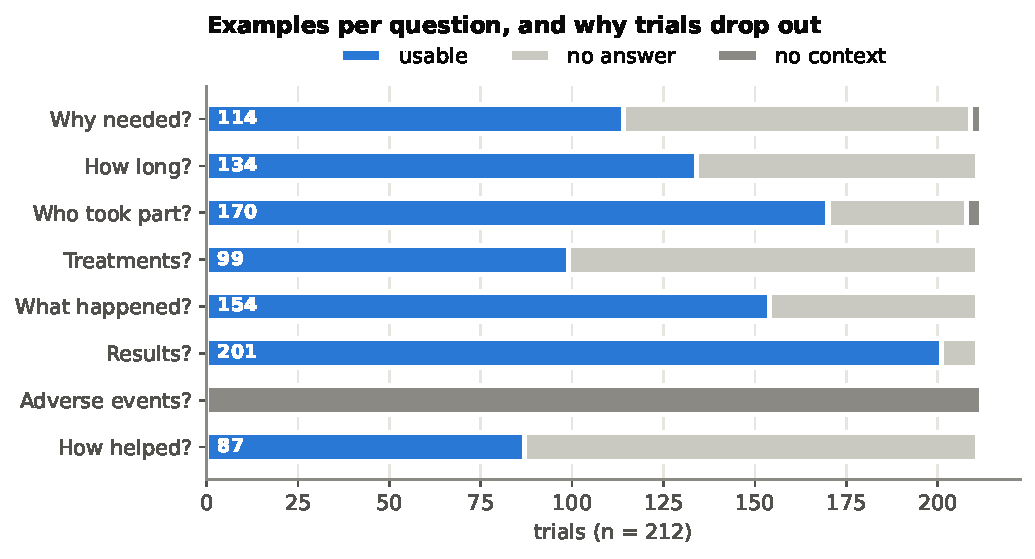
\includegraphics[width=\textwidth]{Figures/results/fig02_question_coverage.pdf}
    \caption[Coverage per question]{Examples per question and reasons for exclusion. The adverse-events question yields none because its mapped section is never extracted.}
    \label{fig:coverage}
\end{figure}

\section{Train, Validation and Test Split}

The examples are split \textbf{by trial} into 70/15/15 shares of the trials (seed 42), so that no trial contributes examples to two splits (Table~\ref{tab:splits}). The original thesis split 85/15 by row, which placed different questions about the same trial in both training and test data. The test set holds 138 examples from 31 trials; Table~\ref{tab:splits_q} gives the split per question. Per-question test cells contain between 12 and 28 examples, too few for claims about individual questions.

\begin{table}[htbp]
    \centering
    \begin{minipage}[t]{0.38\textwidth}
        \centering
        \caption[Dataset split]{Split by trial.}
        \label{tab:splits}
        \begin{tabular}{lrr}
            \toprule
            Split & Trials & Examples \\
            \midrule
            \tabinput{Tables/dataset_splits_body.tex}
            \bottomrule
        \end{tabular}
    \end{minipage}\hfill
    \begin{minipage}[t]{0.58\textwidth}
        \centering
        \caption[Split per question]{Examples per question and split.}
        \label{tab:splits_q}
        \begin{tabular}{lrrr}
            \toprule
            Question & Train & Val & Test \\
            \midrule
            \tabinput{Tables/dataset_splits_per_question_body.tex}
            \bottomrule
        \end{tabular}
    \end{minipage}
\end{table}

\section{How the Targets Differ from the Source}
\label{sec:targets}

Table~\ref{tab:textstats} and Figure~\ref{fig:src_ref} compare the references with their contexts over all 959 examples. Three contrasts define the task.

\begin{itemize}
    \item \textbf{The references are longer than their source.} The median reference has 183 words, the median context 136. Plain-language summarisation here is not compression: the patient summaries explain and expand, for example by defining terms. This matters for the metrics, because short outputs earn little recall.
    \item \textbf{The references are easier to read by the readability formulas.} The median Flesch--Kincaid grade falls from 15.10 in the report context to 10.03 in the references, and the median Flesch Reading Ease rises from 26.28 to 54.73. The source text is also far more variable (standard deviation of the grade 9.18 against 4.30), partly because some sections are tables or lists flattened to text, on which the formulas are unreliable.
    \item \textbf{The references are abstractive.} About 96\% of reference bigrams do not occur in the paired context (Figure~\ref{fig:abstractive}), and \textbf{none of the 959 references occurs verbatim in its context}.
\end{itemize}

The last point has a direct consequence for the extractive question-answering framing of the original thesis, discussed in Section~\ref{sec:extractive}.

\begin{table}[htbp]
    \centering
    \caption[Source vs. reference statistics]{Length, readability and abstractiveness of the report contexts and the plain-language references (all 959 examples). FKGL: Flesch--Kincaid grade level (lower is easier). Flesch Reading Ease: higher is easier.}
    \label{tab:textstats}
    \begin{tabular}{lrrr}
        \toprule
        Statistic & Mean & Median & SD \\
        \midrule
        \tabinput{Tables/dataset_text_stats_body.tex}
        \bottomrule
    \end{tabular}
\end{table}

\begin{figure}[htbp]
    \centering
    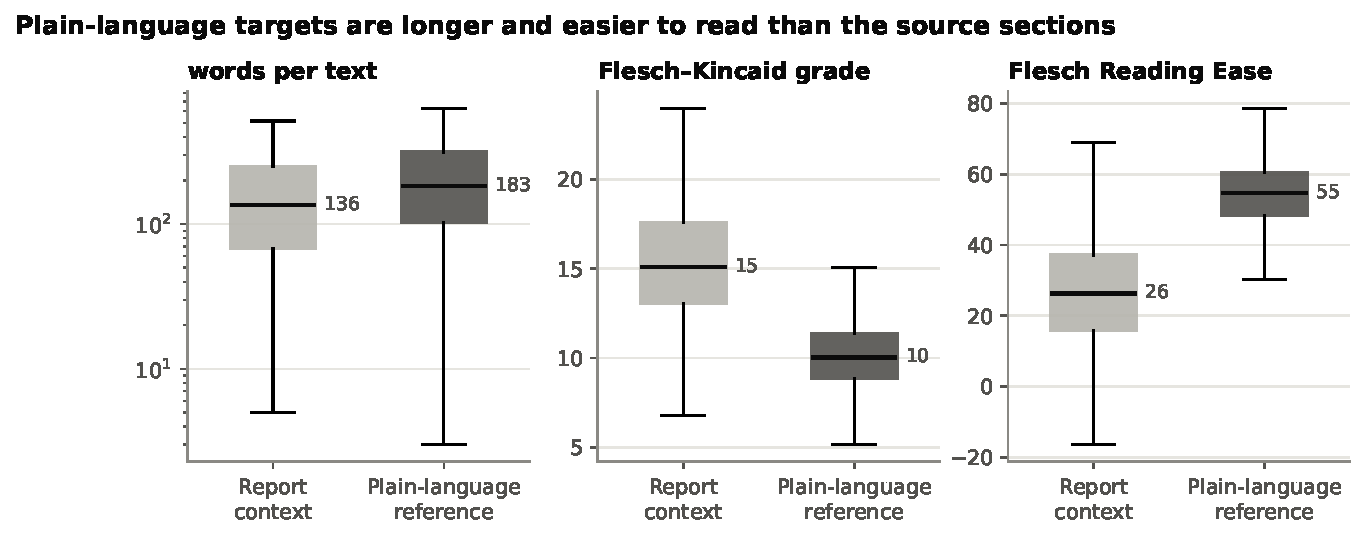
\includegraphics[width=\textwidth]{Figures/results/fig03_source_vs_reference.pdf}
    \caption[Source vs. reference]{Length and readability of report sections vs.\ plain-language references ($n = 959$).}
    \label{fig:src_ref}
\end{figure}

\begin{figure}[htbp]
    \centering
    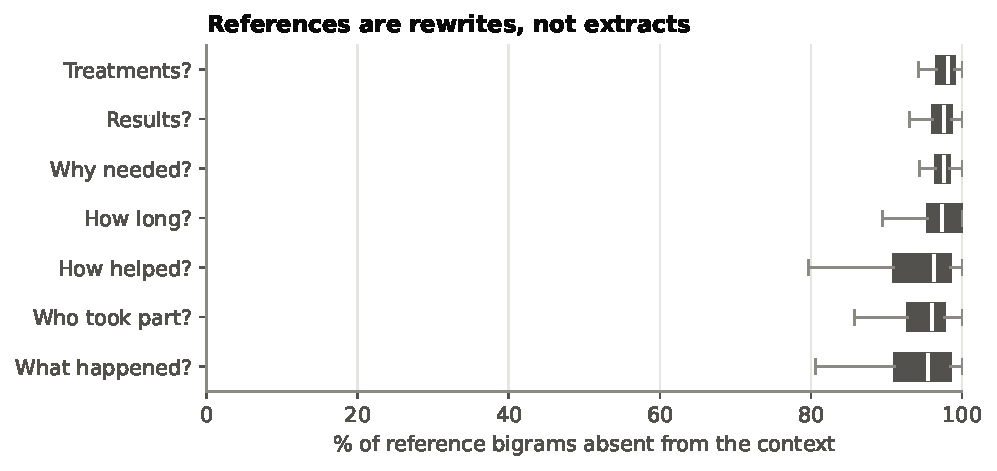
\includegraphics[width=0.85\textwidth]{Figures/results/fig04_reference_abstractiveness.pdf}
    \caption[Reference abstractiveness]{Share of reference bigrams absent from the source, per question.}
    \label{fig:abstractive}
\end{figure}
